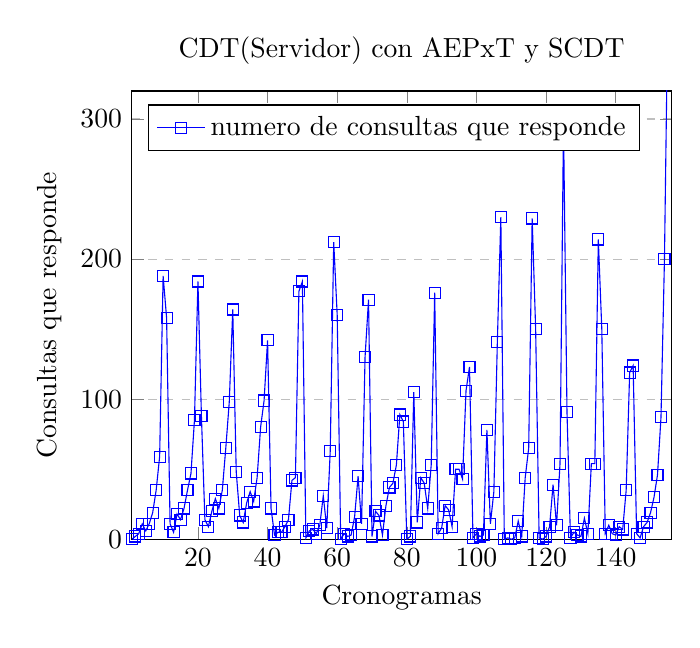
\begin{tikzpicture}
\begin{axis}[
    %CDT = carga de trabajo
    %AEPxT = Algoritmo de Envergadura Probabilista con tiempo de espera
    %SCDT = Seleccion por Carga De Trabajo
    title={CDT(Servidor) con AEPxT y  SCDT},
    xlabel={Cronogramas},
    ylabel={Consultas que responde},
    xmin=1, xmax=156,
    ymin=0, ymax=320,
    xtick={},
    ytick={},
    legend pos=north west,
    ymajorgrids=true,
    grid style=dashed,
]

\addplot[
    color=blue,
    mark=square,
    ]
    coordinates {
   %CARGA DE TRABAJO Servidor
%CARGA DE TRABAJO SERVIDOR
(1,0)
(2,2)
(3,4)
(4,11)
(5,6)
(6,11)
(7,19)
(8,35)
(9,59)
(10,188)
(11,158)
(12,11)
(13,5)
(14,18)
(15,14)
(16,22)
(17,35)
(18,47)
(19,85)
(20,184)
(21,88)
(22,14)
(23,9)
(24,20)
(25,29)
(26,22)
(27,35)
(28,65)
(29,98)
(30,164)
(31,48)
(32,17)
(33,12)
(34,26)
(35,34)
(36,27)
(37,44)
(38,80)
(39,99)
(40,142)
(41,22)
(42,3)
(43,5)
(44,5)
(45,9)
(46,14)
(47,42)
(48,44)
(49,177)
(50,184)
(51,1)
(52,6)
(53,7)
(54,4)
(55,10)
(56,31)
(57,8)
(58,63)
(59,212)
(60,160)
(61,0)
(62,4)
(63,2)
(64,3)
(65,16)
(66,45)
(67,11)
(68,130)
(69,171)
(70,2)
(71,20)
(72,17)
(73,3)
(74,24)
(75,37)
(76,40)
(77,53)
(78,89)
(79,84)
(80,0)
(81,2)
(82,105)
(83,12)
(84,44)
(85,40)
(86,22)
(87,53)
(88,176)
(89,4)
(90,8)
(91,24)
(92,21)
(93,9)
(94,50)
(95,50)
(96,43)
(97,106)
(98,123)
(99,1)
(100,4)
(101,2)
(102,3)
(103,78)
(104,11)
(105,34)
(106,141)
(107,230)
(108,0)
(109,1)
(110,0)
(111,1)
(112,13)
(113,2)
(114,44)
(115,65)
(116,229)
(117,150)
(118,1)
(119,0)
(120,2)
(121,9)
(122,39)
(123,10)
(124,54)
(125,297)
(126,91)
(127,1)
(128,5)
(129,3)
(130,2)
(131,15)
(132,4)
(133,54)
(134,54)
(135,214)
(136,150)
(137,4)
(138,10)
(139,4)
(140,3)
(141,9)
(142,7)
(143,35)
(144,119)
(145,124)
(146,4)
(147,1)
(148,9)
(149,12)
(150,19)
(151,30)
(152,46)
(153,87)
(154,200)
(155,387)
    };
    \legend{numero de consultas que responde}

\end{axis}
\end{tikzpicture}
